\documentclass[sigconf]{acmart}
\settopmatter{printacmref=false}
\usepackage[T1]{fontenc}
%\usepackage{lmodern}
\usepackage[font=small]{caption}
\usepackage{float}
\newtheorem{finding}{Finding}

\usepackage{xspace}
\newcommand{\OMIT}[1]{}
%
% defining the \BibTeX command - from Oren Patashnik's original BibTeX documentation.
\def\BibTeX{{\rm B\kern-.05em{\sc i\kern-.025em b}\kern-.08emT\kern-.1667em\lower.7ex\hbox{E}\kern-.125emX}}
    
% Rights management information. 
% This information is sent to you when you complete the rights form.
% These commands have SAMPLE values in them; it is your responsibility as an author to replace
% the commands and values with those provided to you when you complete the rights form.
%
% These commands are for a PROCEEDINGS abstract or paper.
\copyrightyear{2019}
\acmYear{2019}
\setcopyright{acmlicensed}
\acmConference[WWW '20]{Recomme '18: ACM Symposium on Neural Gaze Detection}{April 20--24, 2020}{Taipei, Taiwan}
\acmBooktitle{WWW '20: ACM Conference on Neural Gaze Detection, June 03--05, 2018, Woodstock, NY}
\acmPrice{15.00}
\acmDOI{10.1145/1122445.1122456}
\acmISBN{978-1-4503-9999-9/18/06}

%
% These commands are for a JOURNAL article.
%\setcopyright{acmcopyright}
%\acmJournal{TOG}
%\acmYear{2018}\acmVolume{37}\acmNumber{4}\acmArticle{111}\acmMonth{8}
%\acmDOI{10.1145/1122445.1122456}

%
% Submission ID. 
% Use this when submitting an article to a sponsored event. You'll receive a unique submission ID from the organizers
% of the event, and this ID should be used as the parameter to this command.
%\acmSubmissionID{123-A56-BU3}

%
% The majority of ACM publications use numbered citations and references. If you are preparing content for an event
% sponsored by ACM SIGGRAPH, you must use the "author year" style of citations and references. Uncommenting
% the next command will enable that style.
%\citestyle{acmauthoryear}

%
% end of the preamble, start of the body of the document source.
\begin{document}
% end of the preamble, start of the body of the document source.

%
% The "title" command has an optional parameter, allowing the author to define a "short title" to be used in page headers.
\title{The Ex-Ante View of Recommender System Design}
%
% By default, the full list of authors will be used in the page headers. Often, this list is too long, and will overlap
% other information printed in the page headers. This command allows the author to define a more concise list
% of authors' names for this purpose.

%
% The abstract is a short summary of the work to be presented in the article.
\begin{abstract}
\end{abstract}

%
% The code below is generated by the tool at http://dl.acm.org/ccs.cfm.
% Please copy and paste the code instead of the example below.
%

%
% Keywords. The author(s) should pick words that accurately describe the work being
% presented. Separate the keywords with commas.
\keywords{Recommender Systems, Beliefs, Decision Theory, Filter Bubbles}

%
% This command processes the author and affiliation and title information and builds
% the first part of the formatted document.

\maketitle

\section{Introduction}

Recommender Systems (RS) have become critical for assisting users in navigating the large choice sets that they face in many online markets. For instance, users have to select from thousands of movies on Netflix, millions of products on Amazon, and billions of videos on YouTube. users in many cases are not aware of most items, let alone have full information about their preferences over them and, to make matters worse, the goods in these markets are usually experience goods whose true utility can only be learned after consumption. Furthermore, users interact with these systems routinely and watch more than one movie on Netflix, buy more than one product on Amazon, and listen to more than one video on YouTube.

Recommender systems have been influential in shaping user choice in these markets with 75\% of movies watched on Netflix and 35\% of page-views on Amazon coming from recommendations. While there are many positive effects from these systems, there is an increasing worry that there are unintended side-effects of recommendation systems. There have been claims that YouTube's recommendation algorithm unintentionally lead to the radicalization of many individuals\footnote{https://www.theatlantic.com/politics/archive/2018/03/youtube-extremism-and-the-long-tail/555350/}, that personalized recommender systems lead users into \textit{filter bubbles} where they get effectively isolated from a diversity of viewpoints or content \cite{pariser2011filter}, and that personalized recommender systems may also lead users to become increasingly homogenized at the same time \cite{chaney2018algorithmic, hosanagar2013will}.

\textbf{Our Model and Contributions} In this paper, drawing from recent work in psychology and decision theory in economics, we first develop a model of user decision-making in the context of large choice sets faced by users in online markets. We then ask how a stylized model of recommendation can shape the behavior of long-lived users and finally ask how the insights from our model can be used to improve recommender system design and to better understand the consequences of these systems.

We focus on understanding the degree to which recommender systems can lead users into \textit{filter bubbles}. Consistent with recent empirical work in the case of movie consumption \cite{nguyen2014exploring}, our model shows that individual consumption behavior over time naturally exhibits patterns consistent with a filter bubble effect \textit{without recommendation}. The key component of our model, drawn from the results of \cite{schulz2019structured}, is that the utilities of similar goods are correlated. This means that when users consume a good and learn its true utility this gives them information about similar goods. Crucially, this not only impacts the underlying belief about the average utility of the good, but also the amount of uncertainty. This learning spill-over induces users to consume goods ``similar" to those they consumed before leading to an increasing narrowing of consumption patterns. This effect is further exemplified when users are \textit{risk-averse}, a concept from economic decision theory where, all else being equal, users have a preference for goods with lower uncertainty to those with higher uncertainty.

We then consider a stylized model of user recommendation and explore how recommendation can affect consumption patterns. We suppose each good is a sum of a common value component and an idiosyncratic component, where the idiosyncratic component is inherently unpredictable given other individual's preferences. We model existing recommendation systems as providing users with information on the common-value component and denote as this as partial recommendation. We consider how user behavior varies as we move from no recommendation to partial recommendation to omniscient recommendation, which is the optimal consumption path for users if they knew the true utility of all the goods in their choice set.

Consistent with \cite{nguyen2014exploring}, we find that partial recommendation increases consumption diversity. However, we also find that partial recommendation increases homogeneity amongst users. 

\textbf{Related Work.}
Recommender Systems

\section{Our Model and Preliminaries}

\subsection{Preliminary on Expected Utility Theory}
[Duarte can do this]

\subsection{Model Setup}
\par
\noindent \textbf{users} We consider a set of users $I$ where each individual $i \in I$ faces the same finite set of $N$ items $\mathcal{N} = \left\{0,1,...,N-1\right\}$. For simplicity, we assume that individuals only derive pleasure from item $n \in \mathcal{N}$ the first time they consume it.

We denote by $u_{in}$ individual $i$'s realized utility from consuming item $n$. In particular, we consider that the realized utility derived from a given item can be decomposed in the following manner:
\begin{align*}
u_{in}= v_{in} + \beta v_n
\end{align*}
where $v_{in}$ denotes an idiosyncratic component -- i.e. user $i$'s idiosyncratic taste for good $n$ --  and $v_{n}$, a common-value component. One can interpret $v_n$ as a measure of how much good $n$ is valued in society in general and, in a sense, $v_{in}$ denotes how $i$ diverges from this overall ranking. The scalar $\beta \in \mathbb{R}_{+}$ denotes the degree to which utilities are idiosyncratic to each individual or common across individuals. If $\beta=0$, it is impossible to generate meaningful predictions of any one's individual preferences based on others, while if $\beta \rightarrow \infty$, every individual has the same preferences. [include some discussion of what this implies about the predictability of a user's preferences]

Stacking utilities in vector-form, we get:
\begin{align*}
{\left(u_{in}\right)}_{n \in \mathcal{N}}=:U_i=V_i+ \beta V
\end{align*}
We stack the idiosyncratic and common-value components as $V_i ={\left(v_{in}\right)}_{n \in \mathcal{N}}$ and $V={\left(v_{n}\right)}_{n \in \mathcal{N}}$.
\par
\noindent \textbf{user Beliefs} We assume that users do not know the realized utilities of the goods before consuming an item.  Formally, user $i$ starts with some beliefs about $U_i$, namely that the idiosyncratic and common-value parts of the utilities are independent -- $V_i \perp \!\!\! \perp V$ -- and that each is multivariate normal. The idiosyncratic utility and common-value utility are distributed as follows:
\begin{enumerate}
\item $V_i \sim \mathcal N (\overline V_i, \Sigma_i)$ 
\item $V \sim \mathcal N(\overline V, \Sigma)$ with $\overline V =0$
\end{enumerate}

We impose the normality assumption for two reasons. The first is that users update their beliefs using Bayesian updating and recall that the normal distribution forms a conjugate family, which allows for simple posterior updates. The second is that it allows us to incorporate an easily interpretable correlation structure between the items.

Keeping with the assumption that $V_i$ represents idiosyncratic deviations from $V$, we assume that, on the population level, prior beliefs $\overline V_i=\left(\overline v_{in}\right)_{n \in \mathcal{N}}$ are drawn independently from a jointly normal distribution, where $\overline v_{in} \sim \mathcal N (0, \overline \sigma^2)$ are i.i.d. These $\overline v_{in}$ denote the prior belief that $i$ holds about the her valuation over good $n$. As people are exposed to different backgrounds, their beliefs about what is good for them also varies and $\overline v_{in}$ denotes this idiosyncrasy at the level of prior beliefs.
\par
\noindent \textbf{user Learning}
When a user consumes a good $n$ they learn the realized utility for that good. In our model we incorporate the idea that learning the utility of good $n$ gives a user information about similar items. We assume that learning about the utility of good $n$ reveals more about the utility associated to items that are closer to it, which captures the idea that trying a product provides more information about similar products than about dissimilar ones.

In order to have a well-defined notion of similarity we need to define a distance function between goods, which we define as:
\begin{align*}
d(n,m):=\min\{ \lvert m - n \rvert ,N - \lvert m - n \rvert \}
\end{align*}
 $m$ and $n$ are the indices of the items in $\mathcal{N}$. We consider that the entry of $n$-th row and the ($m$)-th column of $\Sigma_i$ is given by $\sigma_i^2 \rho^{d(n,m)}$, and that of $\Sigma$ is given by $\sigma^2 \rho^{d(n,m)}$. The scalar $\rho \in [0,1]$ therefore impacts the covariance structure: a higher $\rho$ implies that learning the utility of $n$ is more informative about products nearby. Informativeness, for any $\rho \in (0,1)$, is decreasing in distance. The particular distance function that we utilize leads to this covariance structure being simple, where the $(n,n+1)$-th entry in the covariance matrix is $\rho$ , $(n,n+2)$-th entry is $\rho^2$, etc.
\par
\textbf{user Decision-Making}
We assume the user makes $T$ choices and therefore can only consume up to $T$ items, where $T$ is but a small fraction of $N$. This captures the idea that users are faced with an immense choice set but that ultimately they end up experiencing (and learning) about just a small fraction of it. For tractability we impose that users are myopic and every period consume the product that they have not yet tried ($n_i^t$) that gives them the highest expected utility given the information from past consumption offers ($C_i^{t-1}=(n_i^1,...,n_i^{t-1})$) and their initial beliefs. Any ties are broken uniformly at random. This assumption is critical not only for tractability but also in order to have easily defined benchmarks.
\par
\noindent \textbf{Recommendation}
Our model of recommendation is stylized in order to provide qualitative insights into how recommendation shapes behavior, instead of looking at realistic implementations of recommender systems. We model recommendation as giving users information about the utility of the goods.

We will consider three recommendation regimes:
\begin{enumerate}
\item Partial Recommendation
\item No Recommendation
\item Omniscient Recommendation
\end{enumerate}
The case of primary interest is \textit{partial recommendation} where the recommender observes utilities accrued, but does not know user $i$'s starting beliefs $\overline U_i$. In this case, the recommender knows $V$ but does not know $V_i$.\footnote{We do not consider the acquisition of information for the recommender to know $V$ and suppose that she has sufficient data to learn $V$ before recommendation.} However, the recommender does know the users' beliefs, $\overline V_i$. Thus, at any given period, the recommender provides a personalized recommendation that combines the knowledge of the common value component $V$ with the user beliefs $\overline V_i$. User's beliefs about her valuation of each item become crucial in this case: just providing the user with information about $V$ may change the user's original ranking, but, without considering the user's beliefs, she will not necessarily follow recommendation.

The notion of partial recommendation that we consider is idealized where the recommendation does the Bayesian updating for users. An alternative that is equivalent would be the recommender simply providing $V$ without knowing $\overline V_i$. In this case, the recommendation will be that the user $i$ chooses $r_{it} \in \arg \max_{n \in \mathcal{N} \backslash C_i^T} u_n$, but we assume the recommender provides full information about $V$. For instance, the recommender could display the whole distribution of utilities reported by other users or even its average, which is a good proxy for the common value component.\footnote{
The best item that could recommended with such information if the item with highest common value component. However, in that case, recommending only a single item generates costly Bayesian updating to the user and provides little guidance as to what she should indeed pick as the common value might be of little importance when compared to the idiosyncratic component. Therefore, we assume that the RS reports the whole $V$, which results in higher expected welfare in choices and is not costly to implement.
} The results would be equivalent, but this would shift the burden of Bayesian updating to users.

We further consider two cases that serve primarily as benchmarks. The first is \textit{no recommendation}, where users get no additional information about utilities and make consumption choices based on their beliefs and consumption history. This gives us a benchmark as to how users in our model would behave \textit{without} recommendation so that we can analyze what changes with the introduction of recommendation. The second is \textit{omniscient recommendation} where the recommender knows the true realized utility of each good for each user and can therefore recommend the best remaining good in every period. This gives us a full information benchmark, which is the optimal consumption path for a user if all uncertainty about their preferences was resolved.
\par
\noindent \textbf{Simulation Details}. We analyze our model using numerical simulation since the sequential decision-making component of our model paired with the rich covariance structure between the items make it difficult to characterize optimal user behavior analytically. The Gaussian assumption allows for closed form Bayesian-updating which enables us to simulate our model but does not provide much help in analytical characterizations.

We explore how consumption patterns differ as we consider different recommendation regimes and report representative results from our simulations. We simulate our model over $100$ populations of users with $100$ users per population. For every population and every statistic we calculate, we average over the users in the population to get a representative statistic for this population. A given set of parameters and a population are a single data point in our dataset.

We simulate over a grid of $\gamma, \sigma, \rho, \beta$. When we consider results varying a single parameter, we group the results over the other parameters and consider the differences in value only varying the parameter of interest. We report results for a relatively small $T$. Unless otherwise reported, our results are robust to varying $N$.

\subsection{Discussion of Assumptions}

In this section we provide further discussion of several of the assumptions of our model.

\noindent \textbf{Uncertainty}: We assume that users have underlying uncertainty about the realized utility of the items in their choice sets and as a result face a decision problem under uncertainty. The first justification for this is that environments where recommender systems are commonly deployed, such as on media streaming or e-commerce platforms, contain experience goods. A common assumption in the economics literature is that for experience goods, where users can only observe their realized utility after consumption, users face a decision problem under uncertainty when making consumption choices. The second justification is that, even if users are in an environment where they could observe utilities based on product reviews or introspection, it is prohibitively costly for them to do so in large choice sets.\footnote{Recent empirical work [cite the cameras paper and hodgson-lewis] has shown that, for product search, users engage in a ``zooming in" search strategy in terms of the information they acquire about products before purchasing and only end up acquiring information about a small set of products in a large product space.} Even if they acquired all the information from product reviews, this would only fully resolve uncertainty if individuals did not have idiosyncratic tastes.

This motivates modeling recommendation as providing users \textit{information} in order to reduce their uncertainty.

\noindent \textbf{Large Choice Sets}: We are interested in environments where the number of items in the choice set is very large and users only consume a small number of these items. This is realistic for platforms such as Netflix, Spotify, Amazon, and YouTube where there are sometimes billions of items and users can realistically only consume a handful of these items in their lifetime.

\noindent \textbf{Learning Spillovers}: Users in our environment face a sequential decision-making problem. However, we suppose that individuals are myopic (i.e. consume the item with the highest expected utility, given their beliefs in a single period) in order to maintain tractability. The predominant difficulty in the learning problem they face is not that they need to repeatedly sample a single item in order to learn its value (as in standard multi-armed bandit formulations), but rather that they need to be able to generalize from their experience from consuming one item to other items. After consuming a single item they learn the realized utility of the good.

\indent \cite{schulz2019structured} studies how individuals solve sequential decision-making problems under uncertainty in large choice sets in the context of mobile food delivery orders. They find that individuals engage in similarity-based generalization where learning about the realized utility of a particular good provides them with information about similar goods. Content-based recommender systems exploit a similar idea where, if a user liked one item, then it is also likely that they will like a similar, but different, item as well.

Our model incorporates this observation in a stylized fashion where the degree of information spill-overs is controlled via parameter $\rho$ and we study how the strength of the spill-overs impacts behavior and the effect of recommendation.


\section{Results}

\subsection{Local Consumption}

\begin{figure}
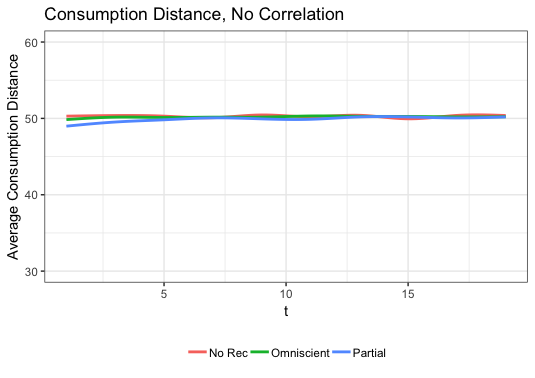
\includegraphics[scale=0.4]{figures/consumption_dist_N_200T_20no_correlation}
\caption{Consumption path with no correlation between utilities}
\label{fig:no_correlation_consumption_path}
\end{figure}

\begin{figure}
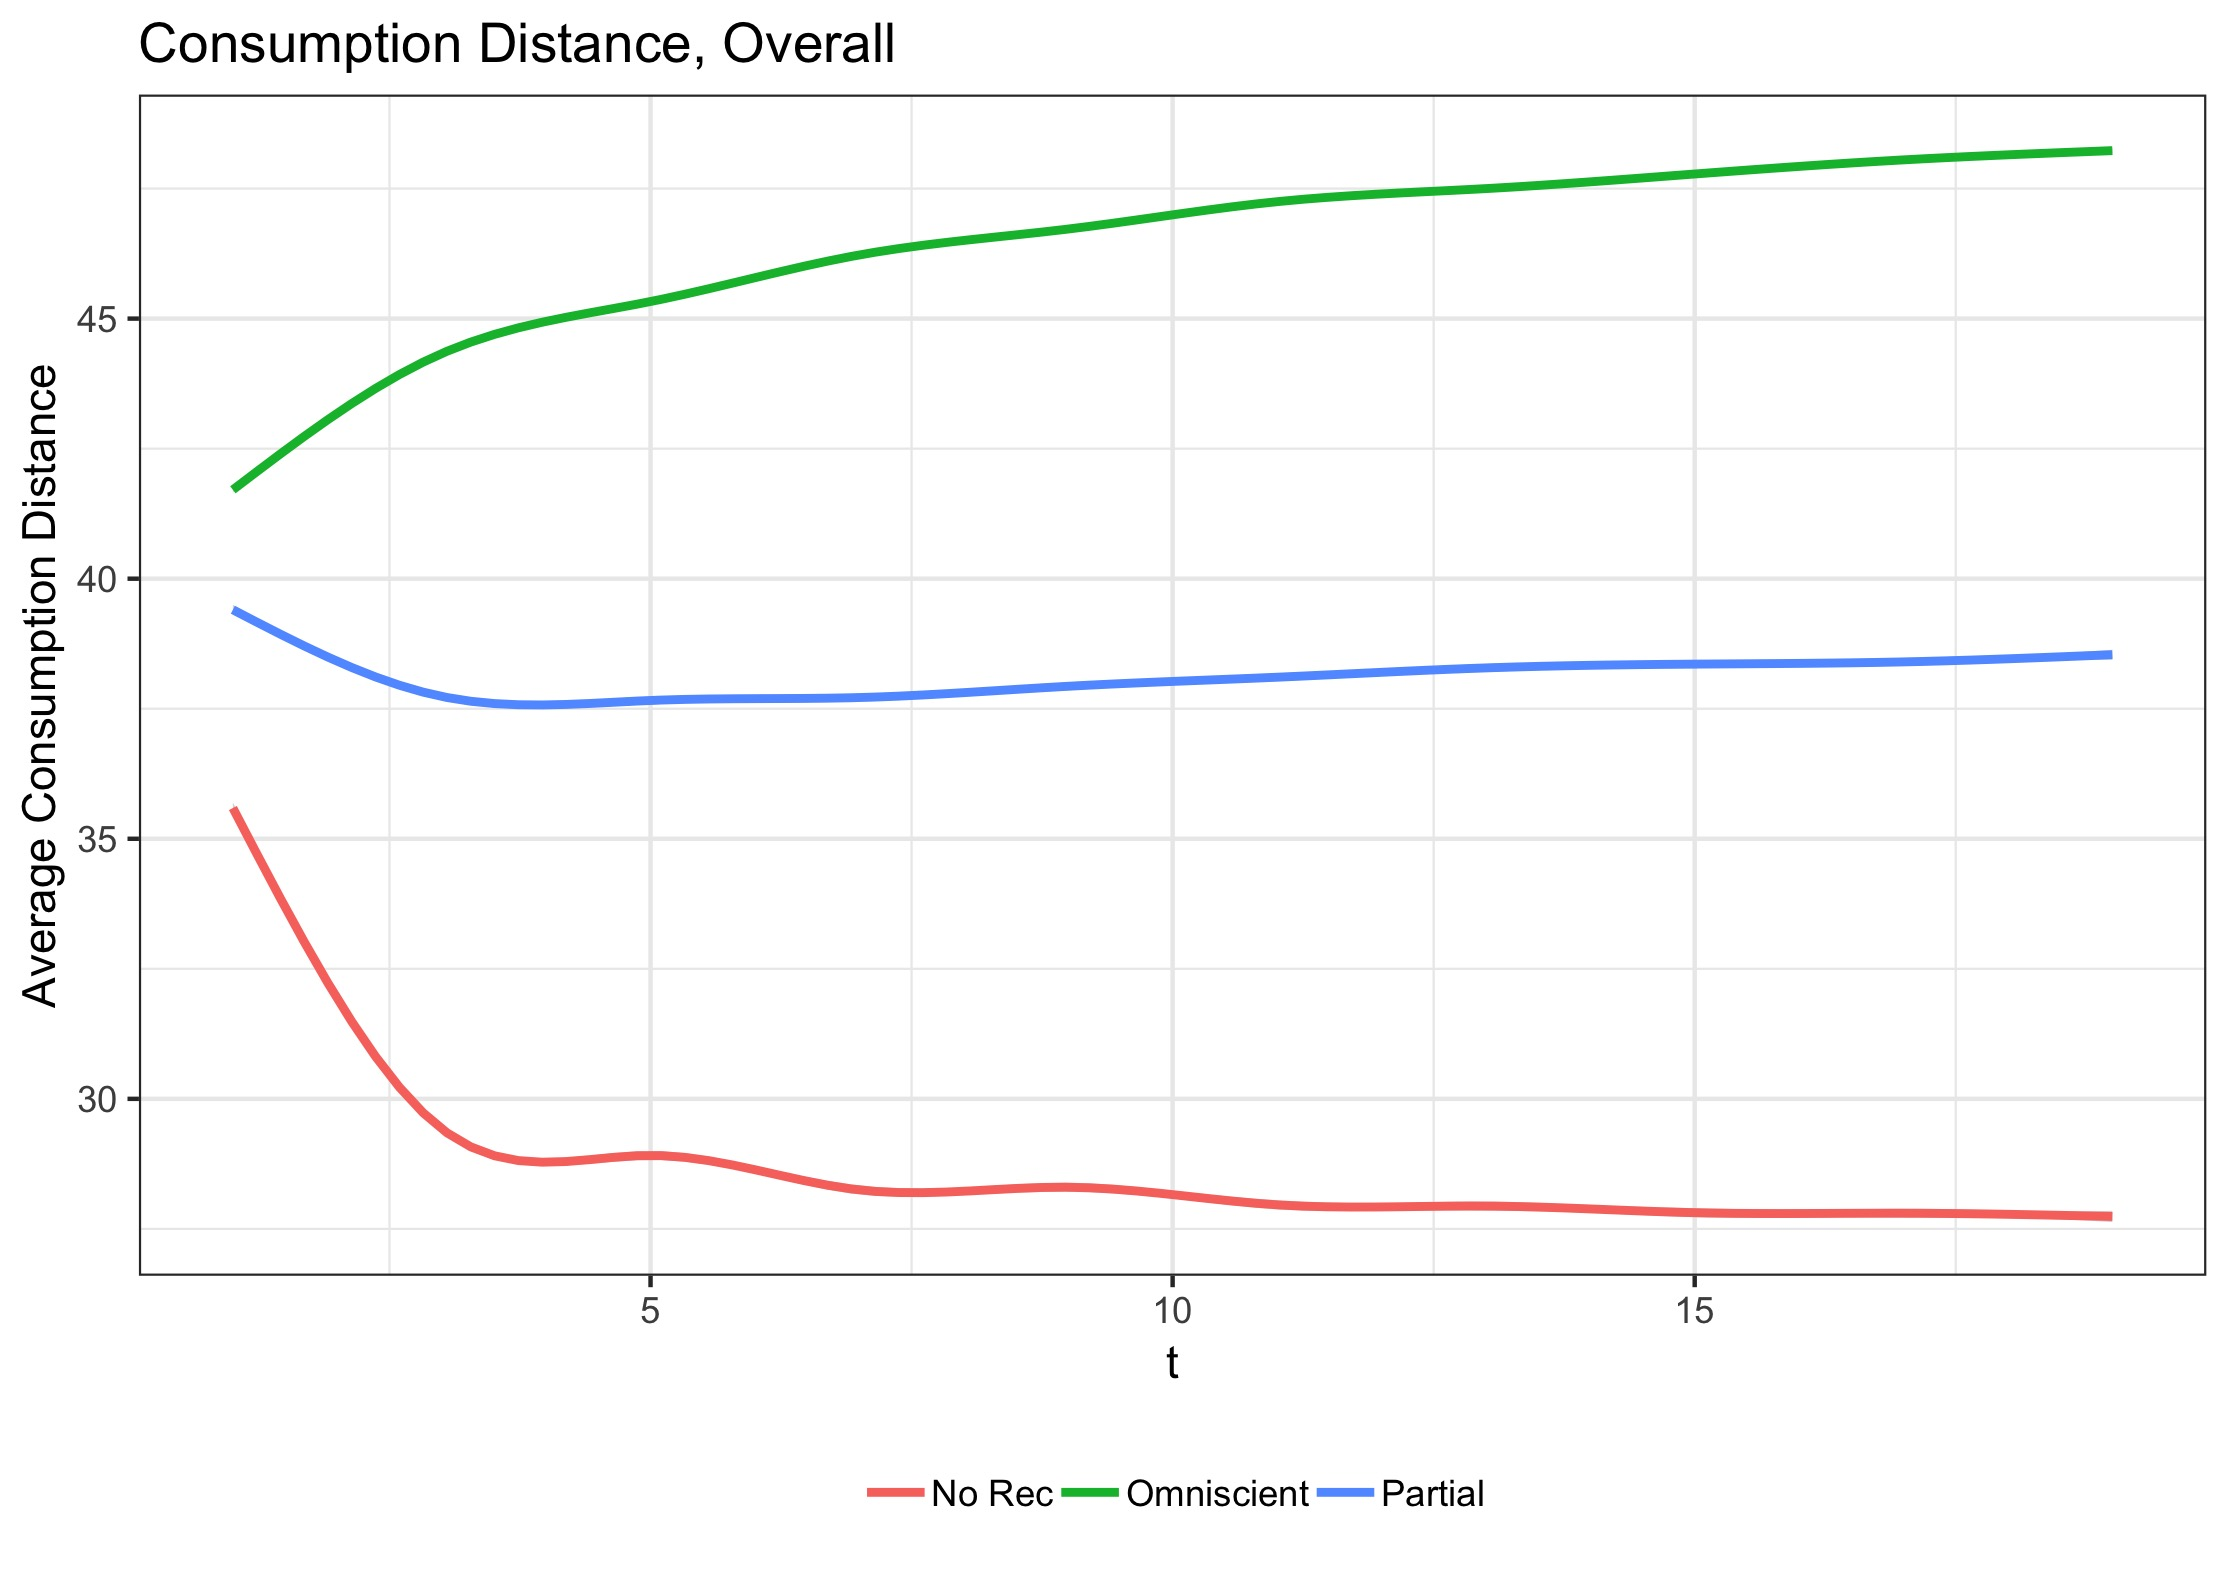
\includegraphics[scale=0.1]{figures/consumption_dist_N_200T_20_overall}
\caption{Consumption path between Recommendation Regimes}
\label{fig:consumption_path_between_regimes}
\end{figure}

We characterize ``filter bubble" effects in our model as the degree to which users engage in \textit{local consumption}. We define local consumption in terms of the average consumption distance between the items consumed by the representative user at time $t-1$ and $t$. We compare the average movement within the product space across different recommendation regimes and associate lower average distance with more local consumption.

\begin{finding}\label{finding_local_consumption}
The impact of recommendation on local consumption:
\begin{enumerate}
\item When $\rho = 0$, there is no difference in consumption distance between the three recommendation regimes.
\item When $\rho > 0$, no recommendation induces more local consumption than both partial and omniscient recommendation. This effect is amplified as $\rho$ increases as well as when users are more risk averse ($\gamma$ increases)
\end{enumerate}
\end{finding}

First, Figure \ref{fig:no_correlation_consumption_path} shows that, when $\rho = 0$, there is no difference in consumption distance between the three regimes. This is due to the fact that when $\rho = 0$, there is no reason that items that are close in the product space should have similar utilities and so the optimal consumption path does not depend on the similarity of the items. However this also means that users in the no recommendation regime do not learn anything about neighboring goods and so there is limited path-dependence in consumption.

Figure \ref{fig:consumption_path_between_regimes} shows that, when $\rho > 0$, both partial and no recommendation lead to increasingly local consumption compared to the benchmark omniscient case. Further, the average consumption path between periods is \textit{decreasing} for the no recommendation case whereas it is \textit{increasing} for the omniscient case. Partial recommendation decreases the degree of local consumption but not as much as the omniscient benchmark. Due to the correlation of utilities, the omniscient consumption path exploits this and leads to the consumption of more similar products than in the case when $\rho = 0$. However, since these spillovers also impact user learning in the no recommendation case, users \textit{over-exploit} this and increasingly consume products similar to good products that they have consumed before. This is further illustrated by Figure \ref{fig:local_consumption_across_rho} which shows how the consumption paths between omniscient and no recommendation vary as $\rho$ increases.

Finally, this effect is further amplified as the level of risk aversion, $\gamma$, increases. Figure \ref{fig:no_rec_risk_aversion} shows how drastically the degree of local consumption increases as $\gamma$ increases. This is due to the fact that the spillovers not only affect the mean expected belief about quality but also the degree of uncertainty. Local consumption therefore leads to users to have less uncertainty about certain areas of the product space and risk aversion may lead them to increasingly consume these products.

\begin{figure*}
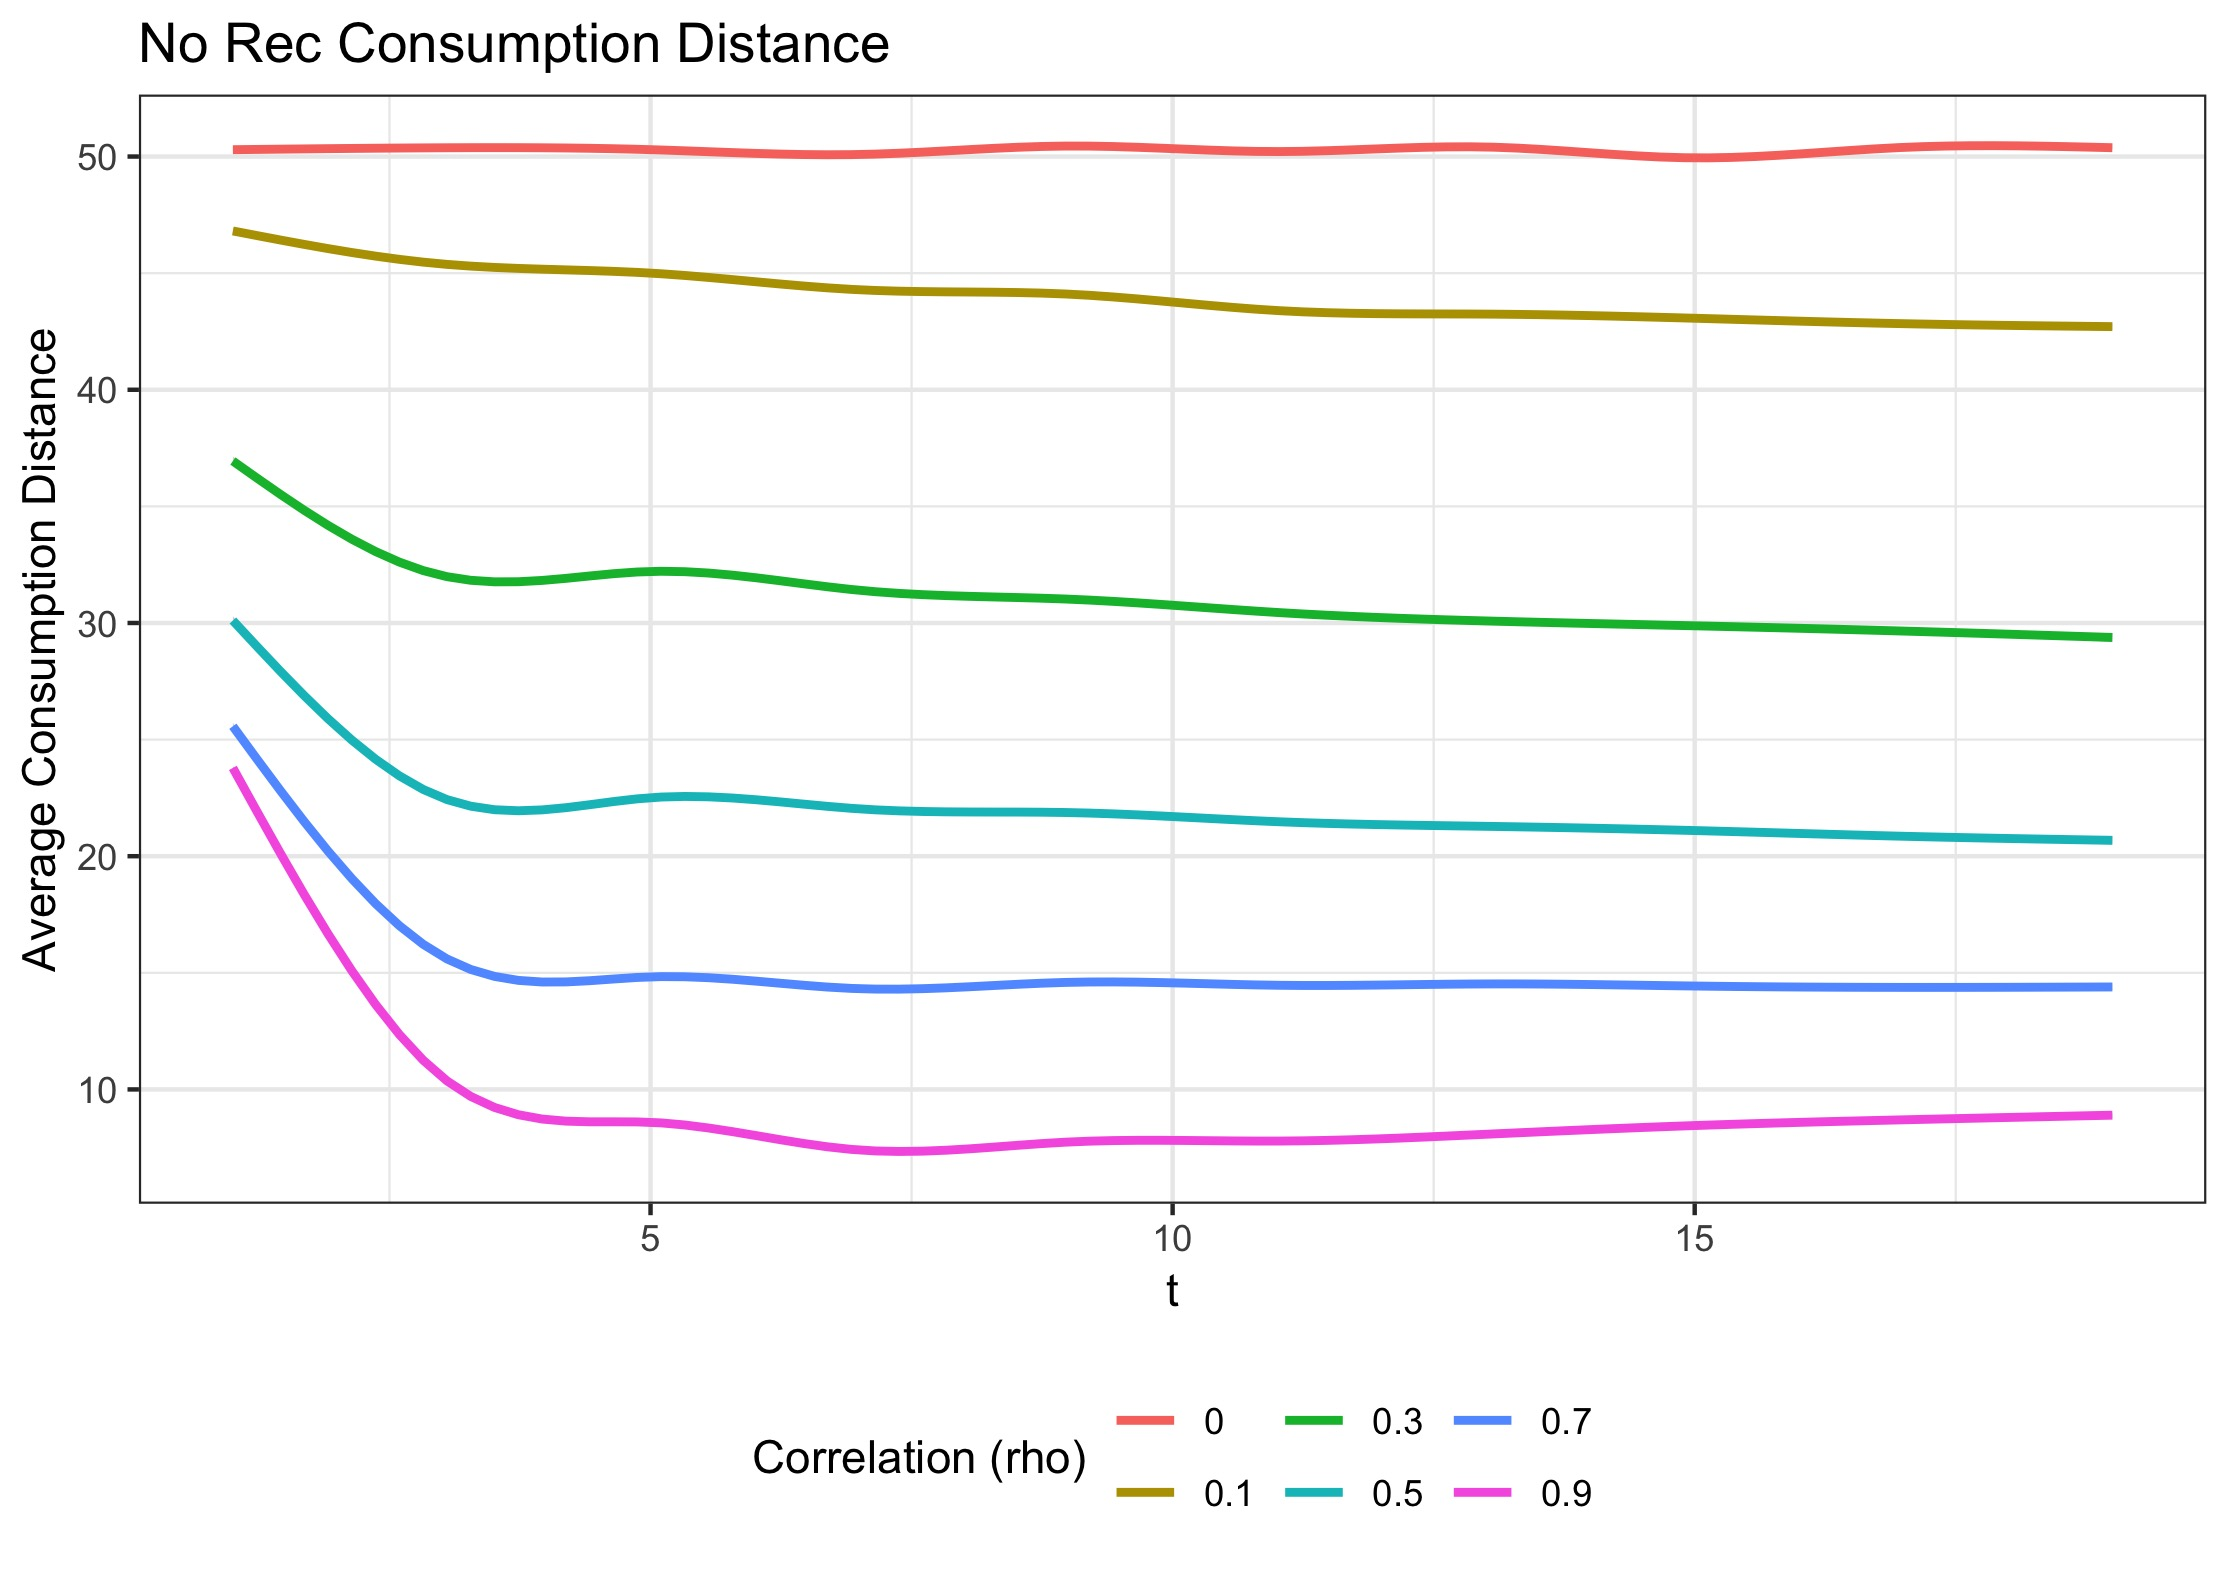
\includegraphics[scale=0.1]{figures/consumption_dist_N_200T_20_no_rec_rho}
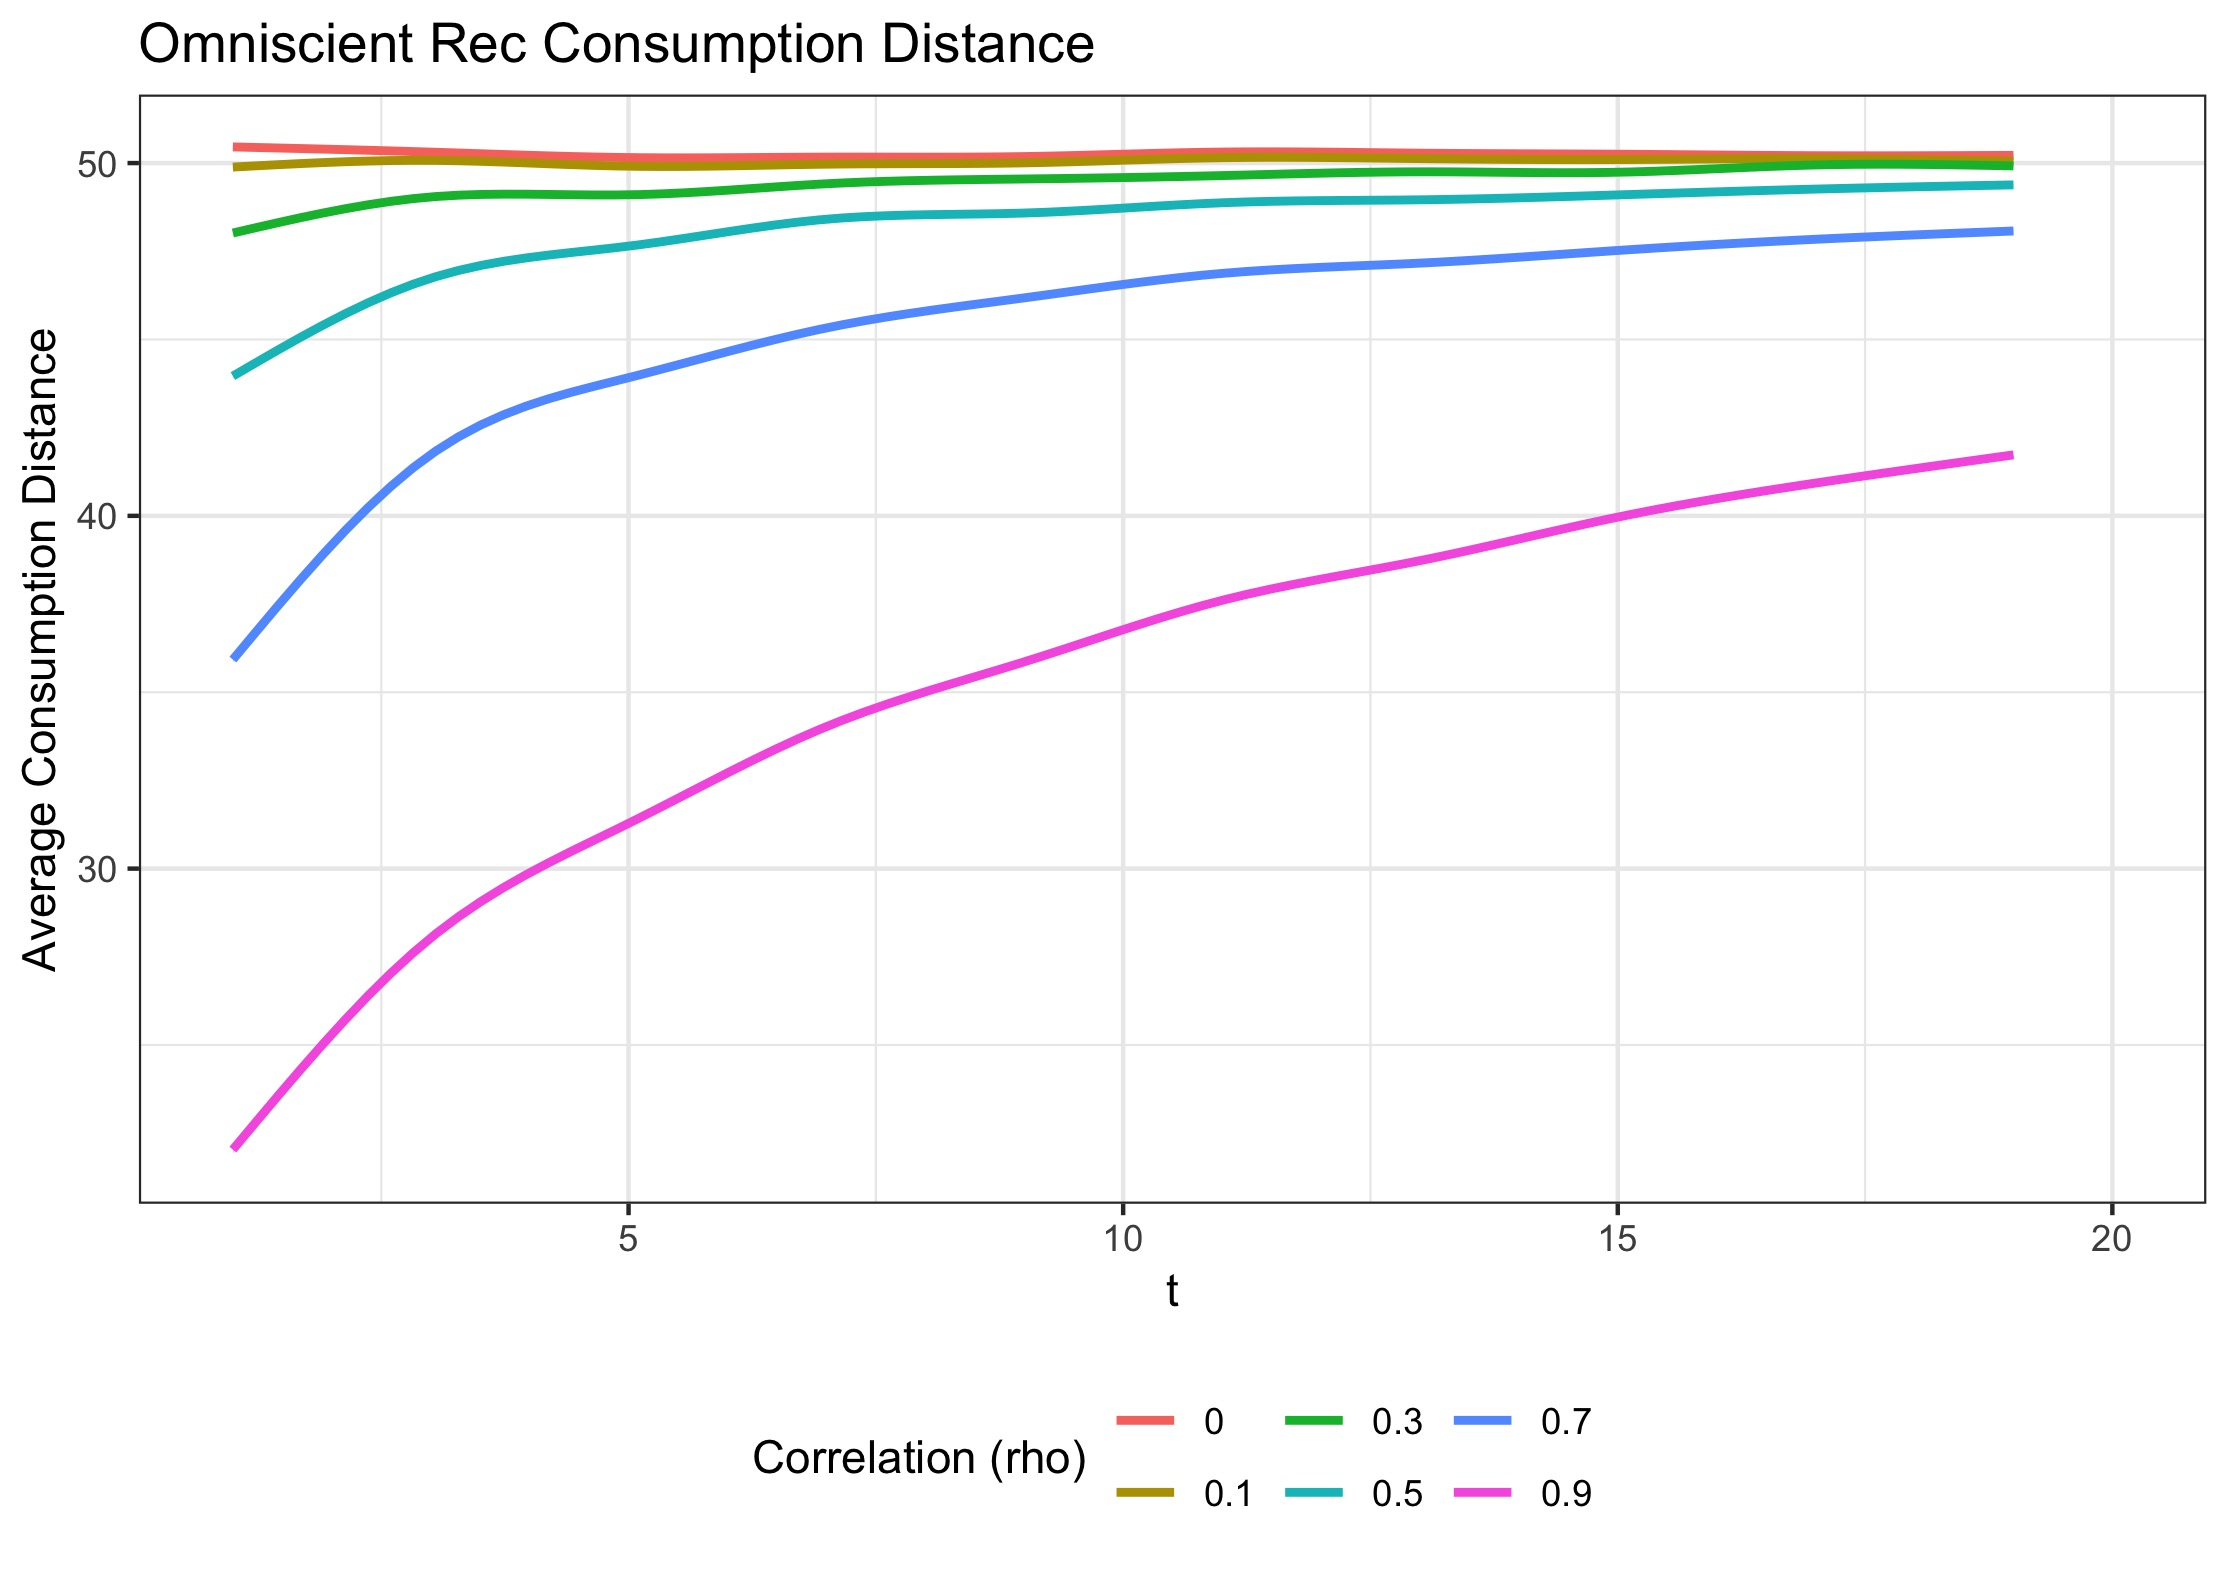
\includegraphics[scale=0.1]{figures/consumption_dist_N_200T_20_omni_rho}
\caption{Extent of Local Consumption for No Recommendation (Left) and Omniscient Recommendation (Right)}
\label{fig:local_consumption_across_rho}
\end{figure*}

\begin{figure}
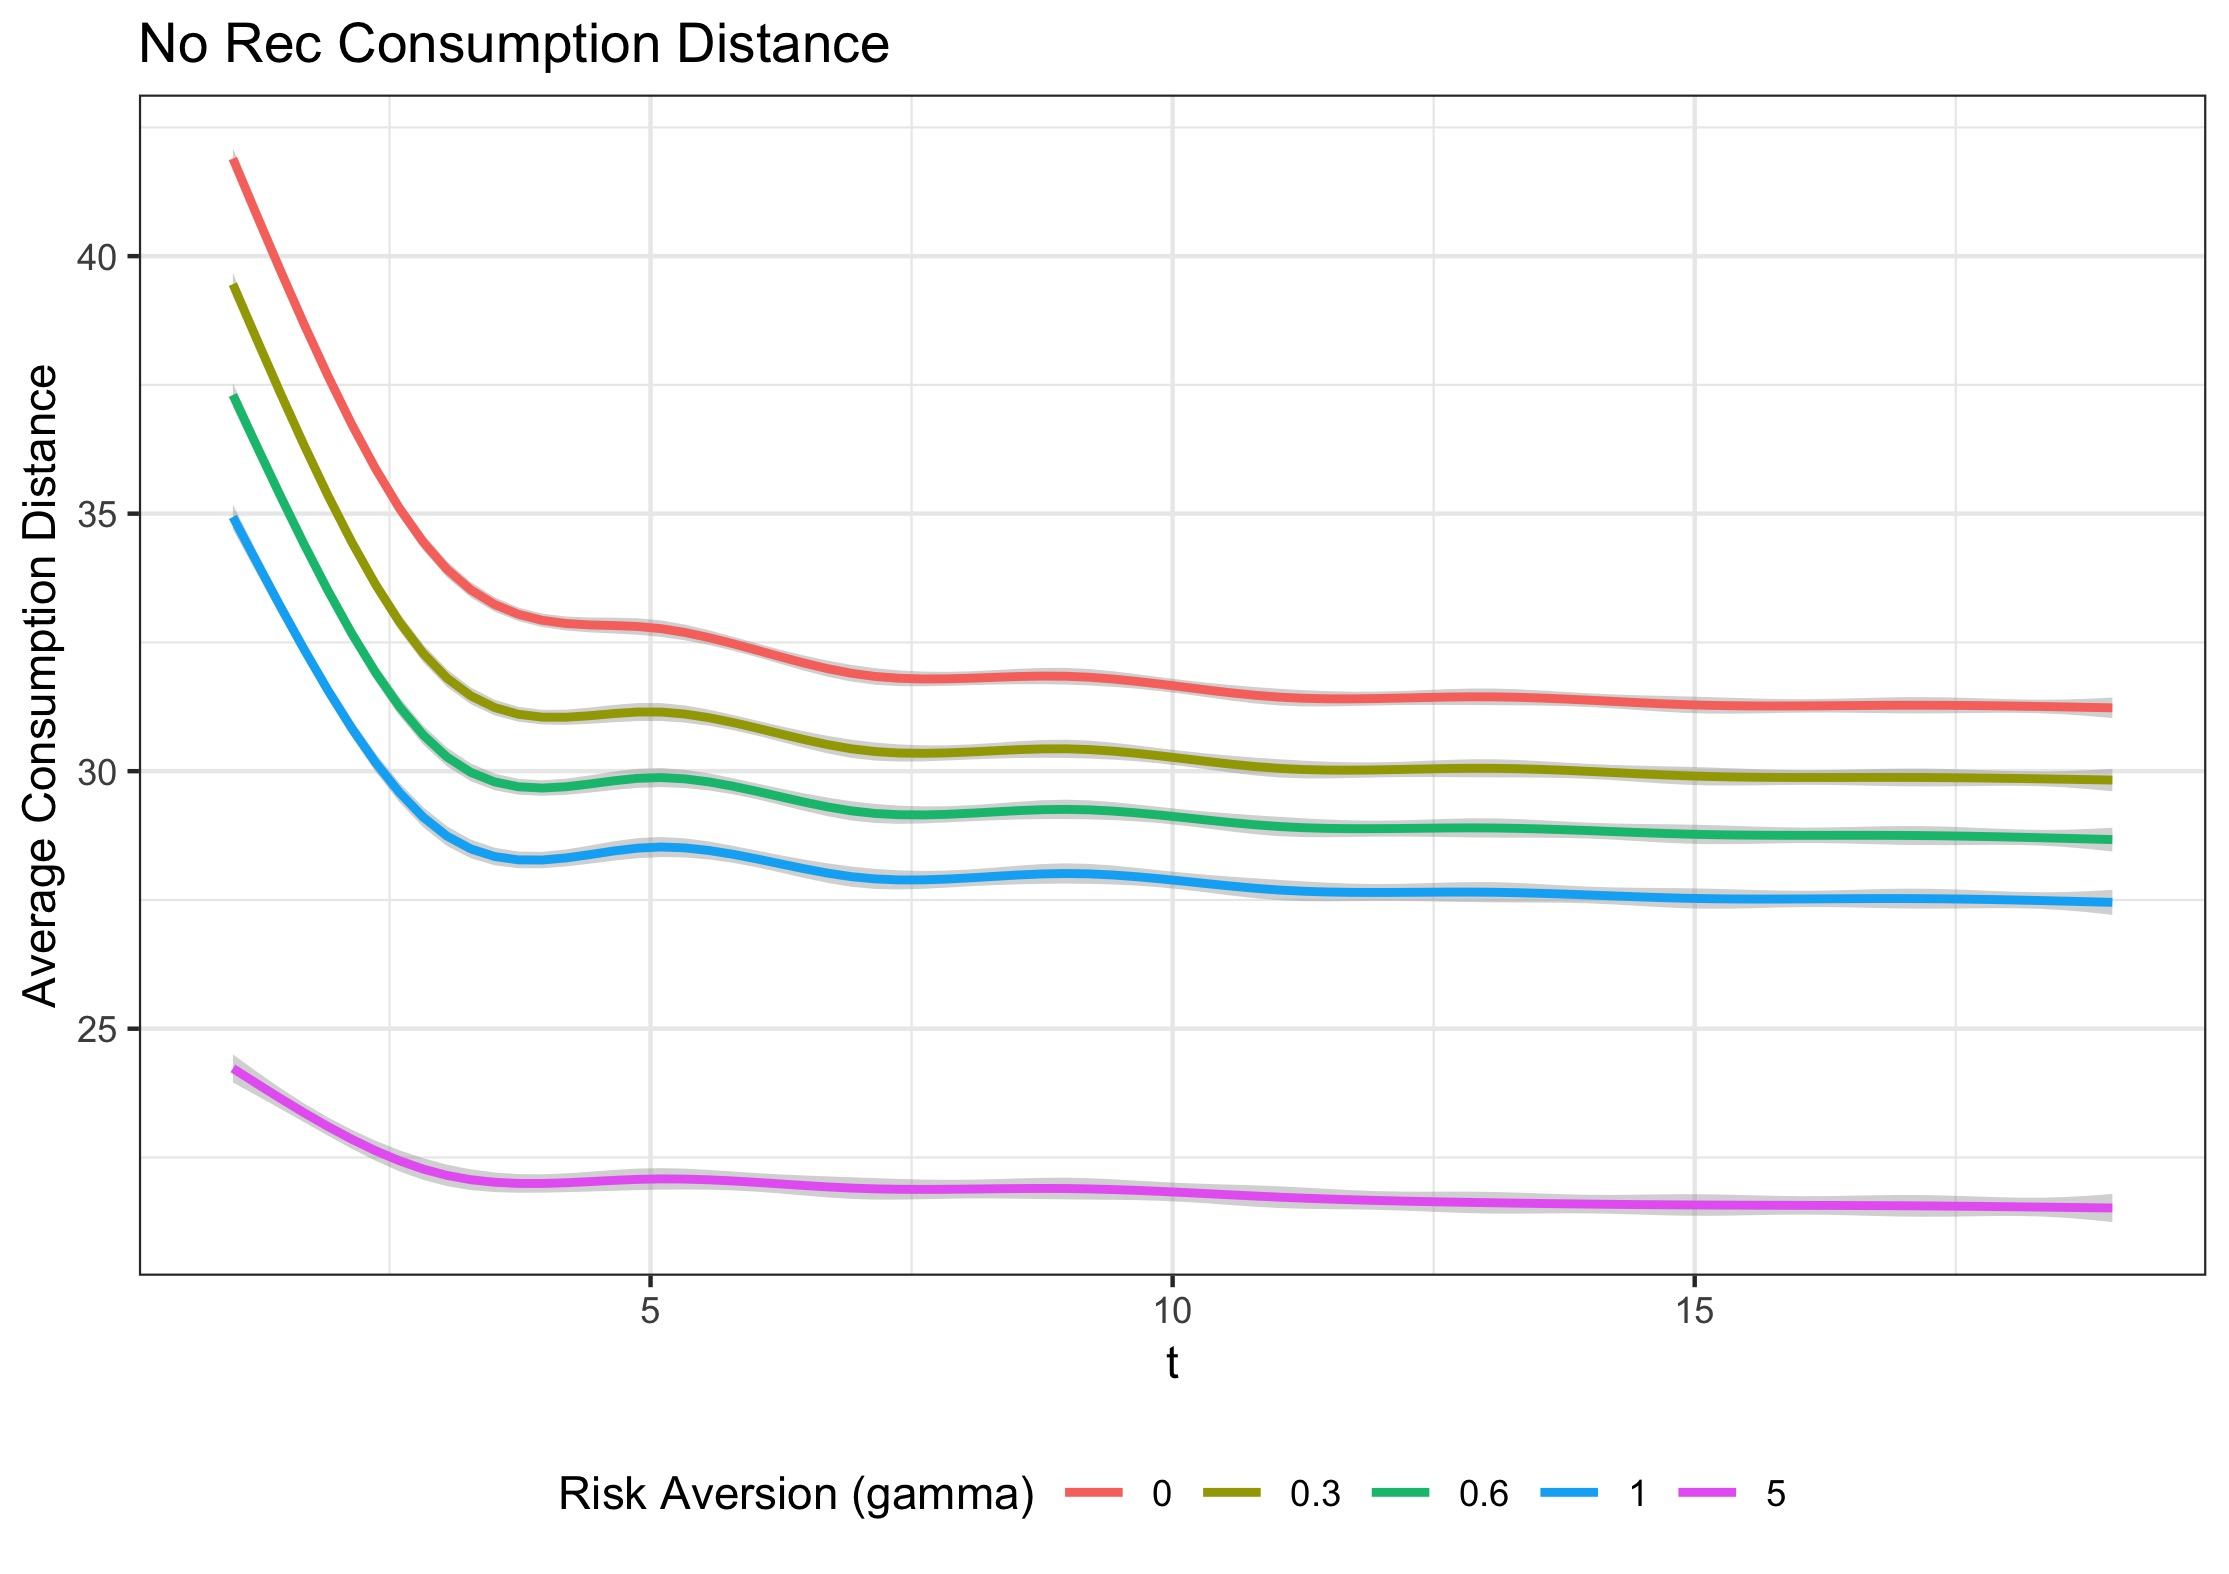
\includegraphics[scale=0.1]{figures/consumption_dist_N_200T_20_no_rec_alpha}
\caption{The Effect of Risk Aversion on Local Consumption}
\label{fig:no_rec_risk_aversion}
\end{figure}

\subsection{User Welfare and Product Diversity}

In this section we primarily focus on the impact of recommendation on the welfare on users as well as the overall diversity of the items that they consume.
user's \textit{ex-post} welfare is the average of realized utilities, to control for the effect of $T$, and is defined as follows:
\begin{align*}
W_i=\frac{1}{T}\sum_{n \in C_i^T} u_{in}
\end{align*}
While in the previous section we looked at the distance between consecutive goods, we also define a diversity measure that is defined over the entire consumed set. We utilize a diversity metric common in the literature (e.g. \cite{ziegler2005improving}) which is the average normalized pairwise distance between the consumed products:
\begin{align*}
D_i =\frac{1}{N} \frac{1}{T (T-1)}\sum_{n,m \in C_i^T: n \ne m} d(n,m)
\end{align*}

\begin{finding}\label{finding_diversity}
The impact of recommendation on product diversity:
\begin{enumerate}
\item When $\rho = 0$, product diversity is the same across all three recommendation regimes.
\item When $\rho > 0$, product diversity decreases across all recommendation regimes but decreases the most in the no recommendation regime. This effect is amplified as $\rho$ increases as well as when users become more risk-averse.
\end{enumerate}
\end{finding}

As before, when there is no correlation between utilities product diversity is the same across different recommendation regimes. The over-exploitation of the learning spillovers when $\rho > 0$ leads to product diversity being lowest in the no recommendation regime. Figure \ref{fig:diversity_correlation} shows how diversity varies across recommendation regimes and the level of $\rho$ and Figure \ref{fig:risk_aversion_diversity} shows how diversity varies as risk aversion levels change. 

\begin{finding}\label{finding_welfare_gap}
The welfare gap between no recommendation and partial recommendation as well as no recommendation and omniscient recommendation is decreasing in $\rho$.
\end{finding}
However, interestingly, the decrease in diversity is \textit{not} associated with a decline in welfare. In fact, welfare stays roughly the same in the omniscient case and slightly increases for the partial recommendation case. The welfare gap between the no recommendation case and the other two cases \textit{decreases} as the diversity gap increases.

\begin{finding}\label{finding_diversity_welfare_corr}
Without recommendation, diversity and welfare are:
\begin{enumerate}
\item Negatively correlated when users have no risk-aversion
\item Uncorrelated when users have high levels of risk-aversion
\end{enumerate}
\end{finding}

Figure \ref{fig:diversity_welfare_ra} shows how diversity and welfare correlate for the no recommendation case. When there is no risk-aversion then there is a negative correlation between welfare and diversity. This is since, with no risk-aversion, in a given period a user will select the good that they currently believe has the highest expected value. High product diversity in this case can arise from a user who consumes a bad item and updates her beliefs about nearby items negatively. As a result, in the next period she will pick an item far away in the product space from the item that she consumed previously. If the item that she had consumed was ``good", then she is more likely to pick a nearby item. The learning spillovers therefore lead to high product diversity being negatively correlated with welfare.

\begin{figure}
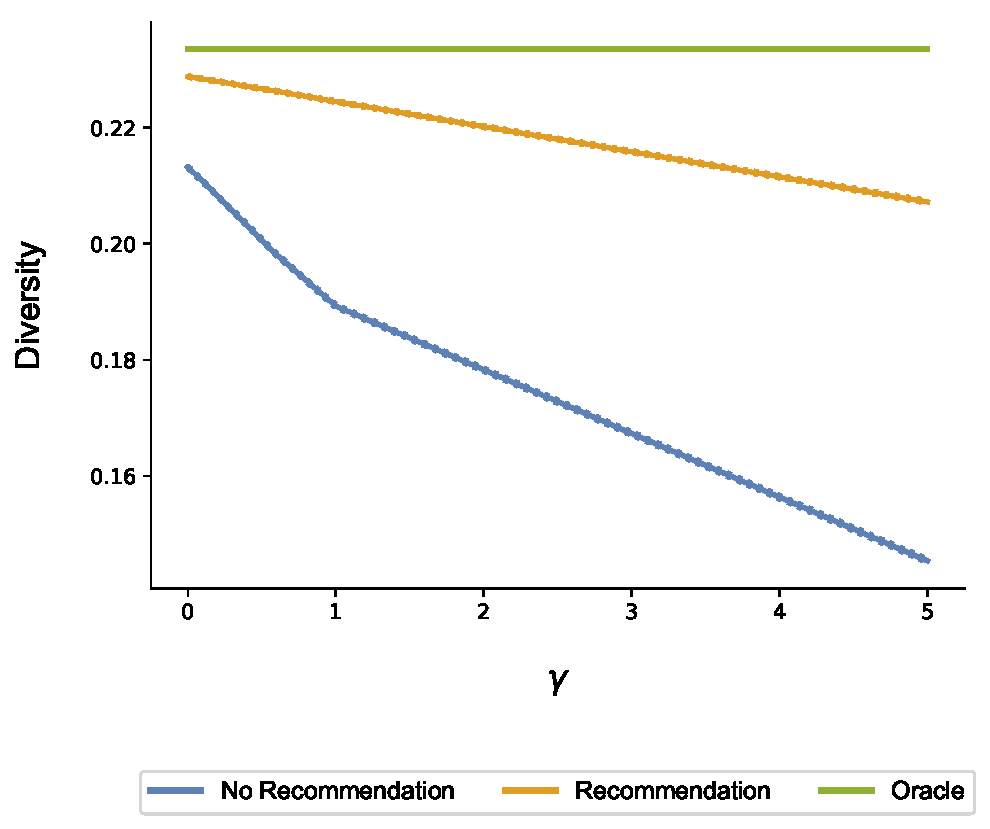
\includegraphics[scale=0.1]{figures/gamma_diversity_N_200_T_20}
\caption{Risk Aversion and Diversity}
\label{fig:risk_aversion_diversity}
\end{figure}

This only happens since $\gamma = 0$ leads to users only caring about the expected value of the good. However, as we saw in Findings \ref{finding_local_consumption} and \ref{finding_diversity}, increasing $\gamma$ can lead to lower diversity and increasingly local consumption due to the fact that the degree of uncertainty now impacts users' choices. This weakens the negative relationship between diversity and welfare since both negative and positive experiences with a good reduce uncertainty about surrounding goods. This leads to the inverted-U shape found in Figure \ref{fig:diversity_welfare_ra} when $\gamma$ is relatively large (e.g $\gamma = 5$).

\begin{figure*}
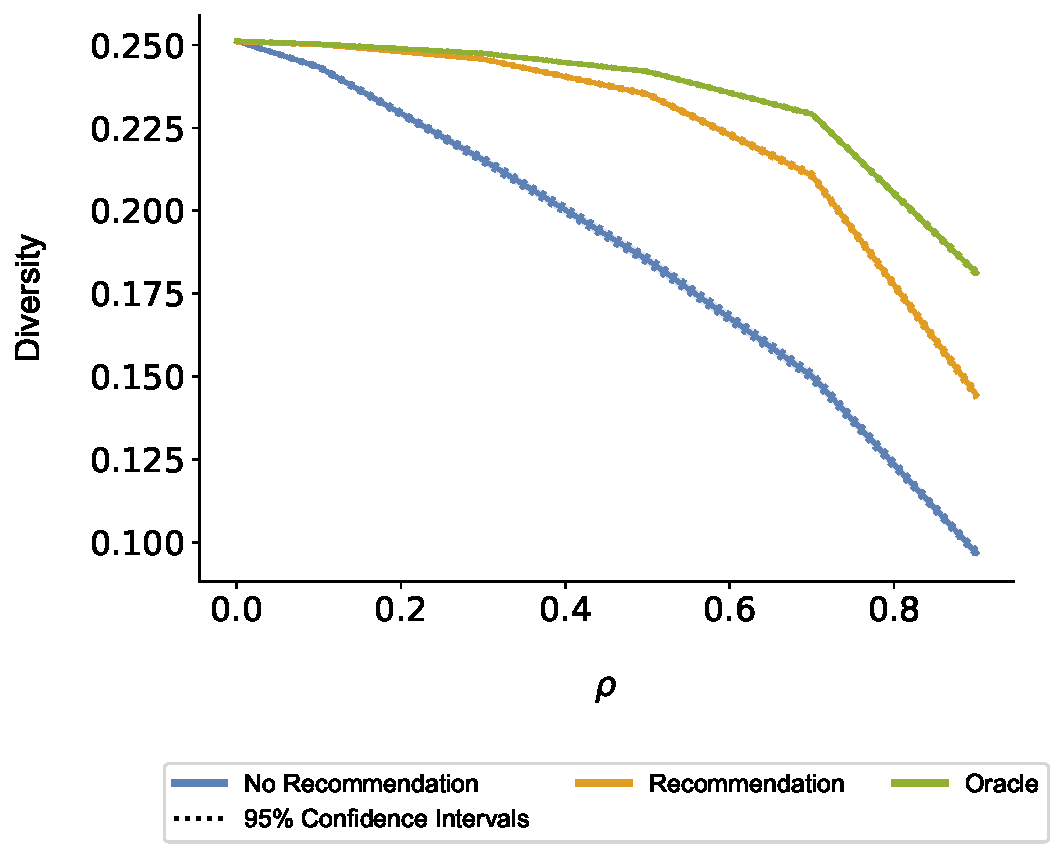
\includegraphics[scale=0.1]{figures/rho_diversity_N_200_T_20}
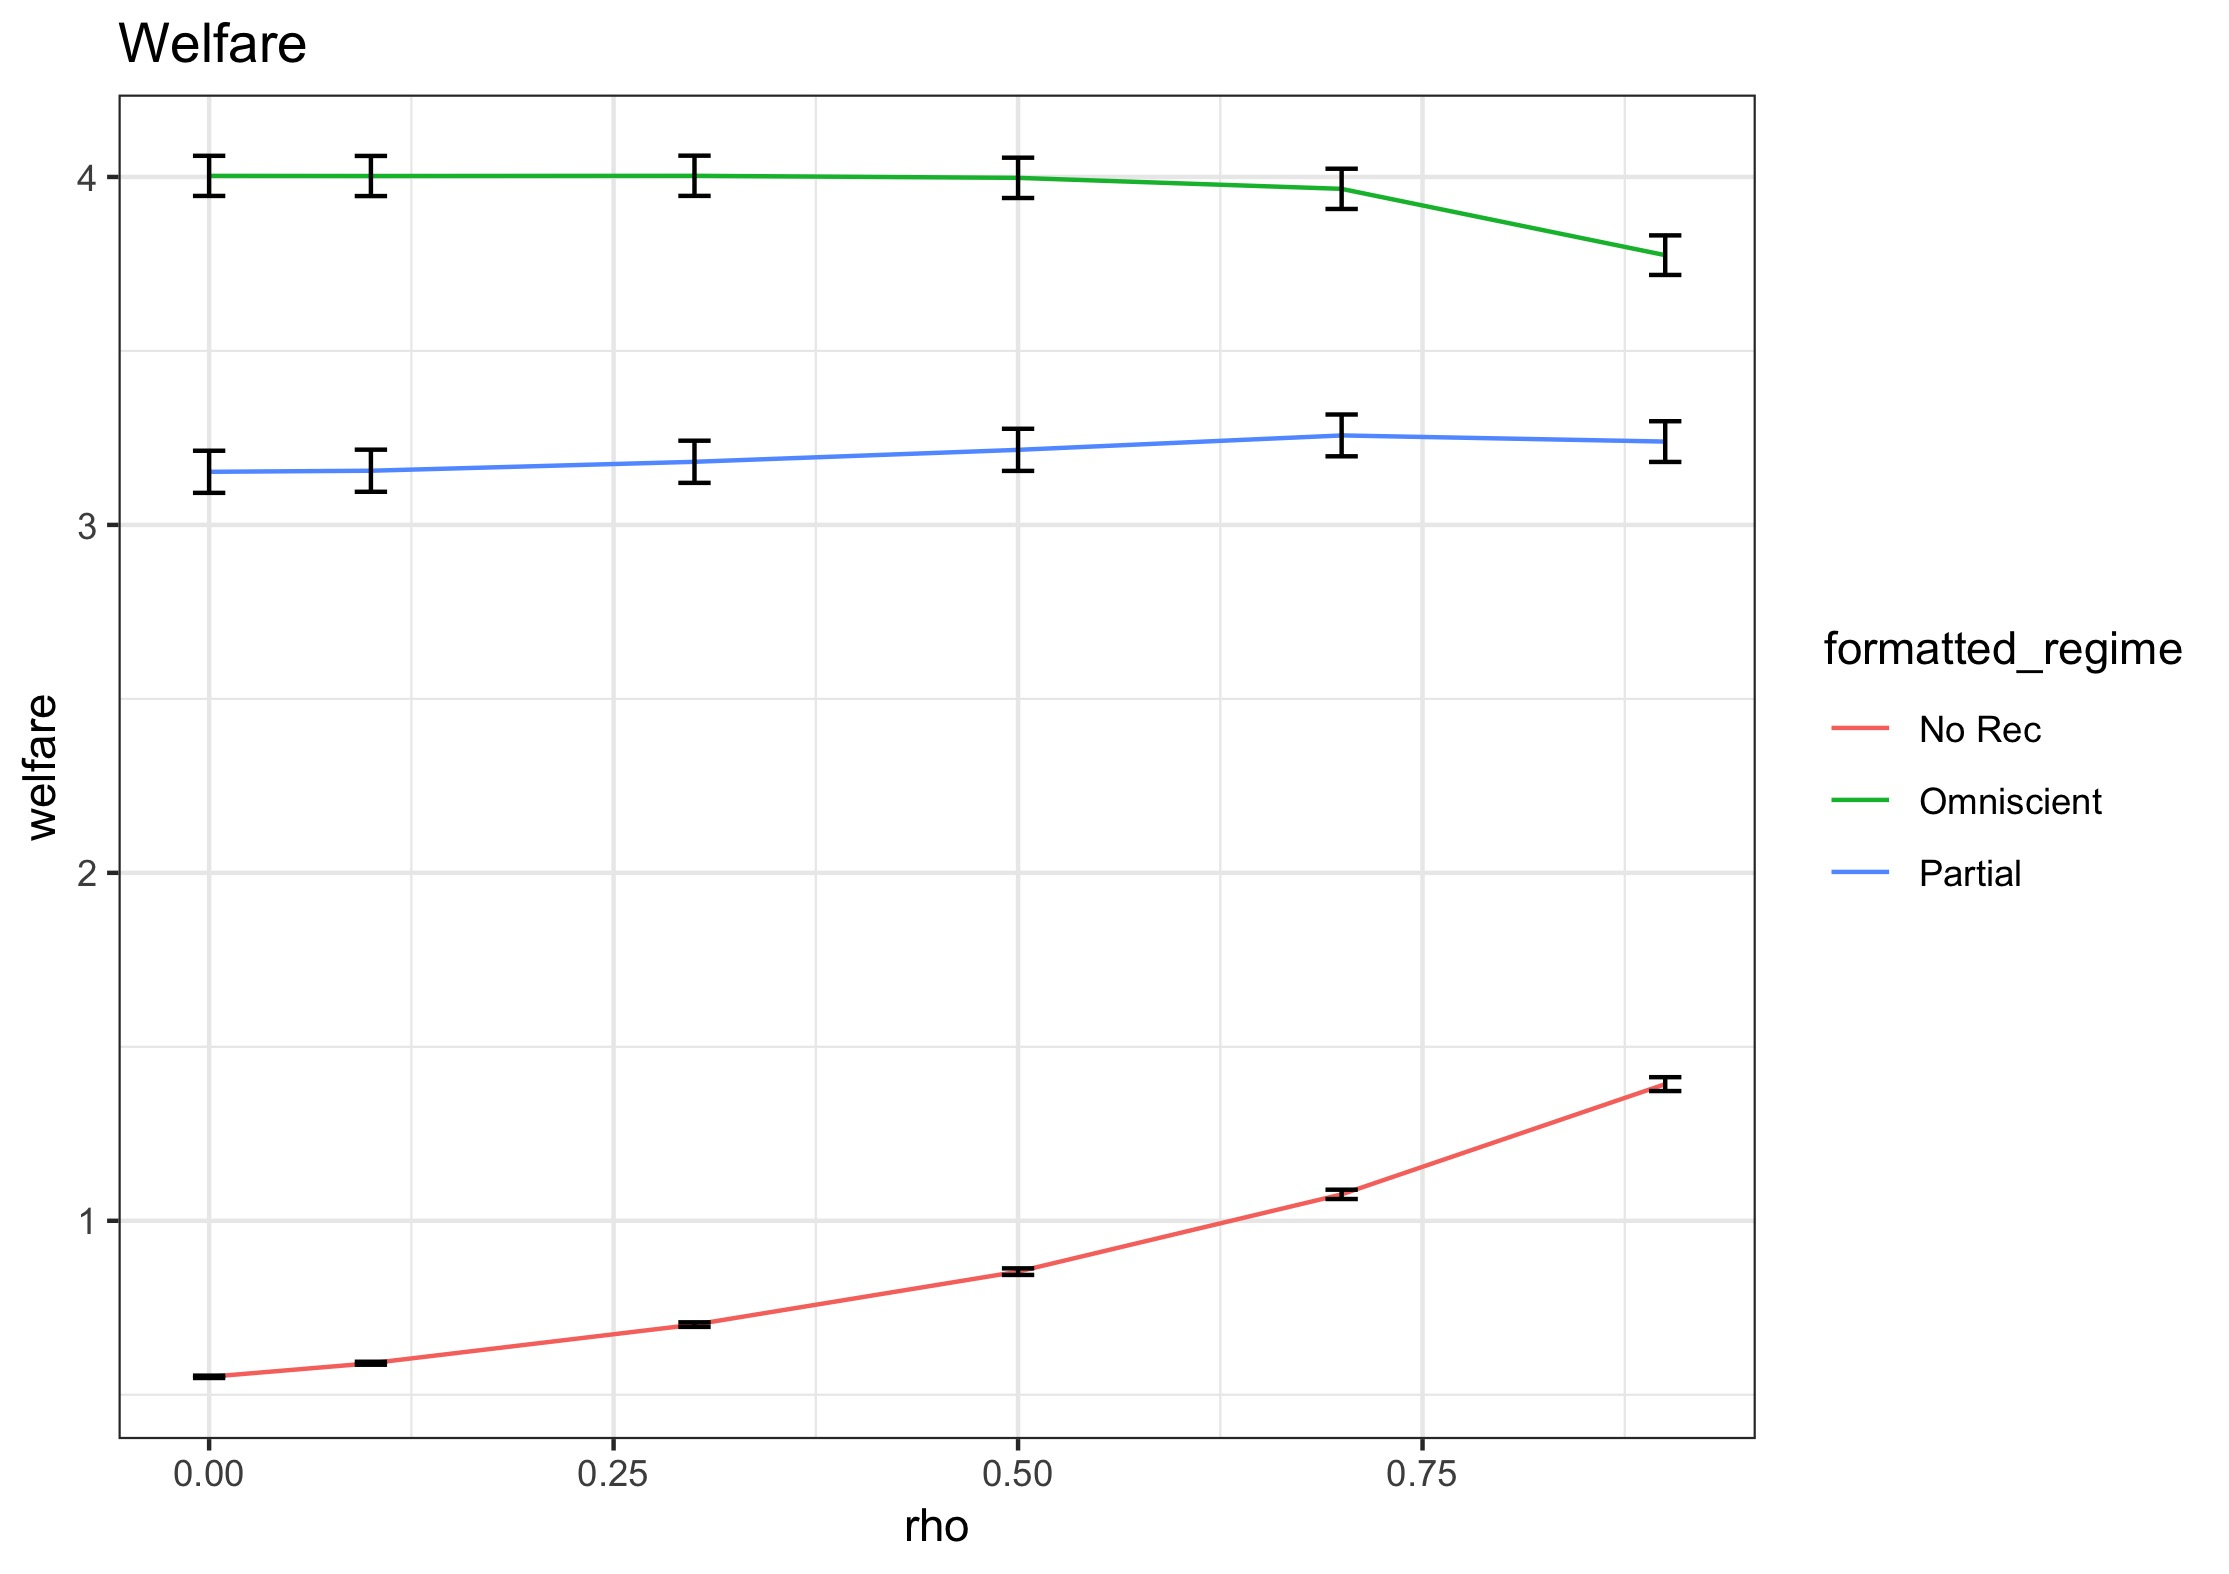
\includegraphics[scale=0.1]{figures/rho_welfare_N_200_T_20}
\caption{Welfare, Diversity, and Correlation}
\label{fig:diversity_correlation}
\end{figure*}

\begin{figure*}
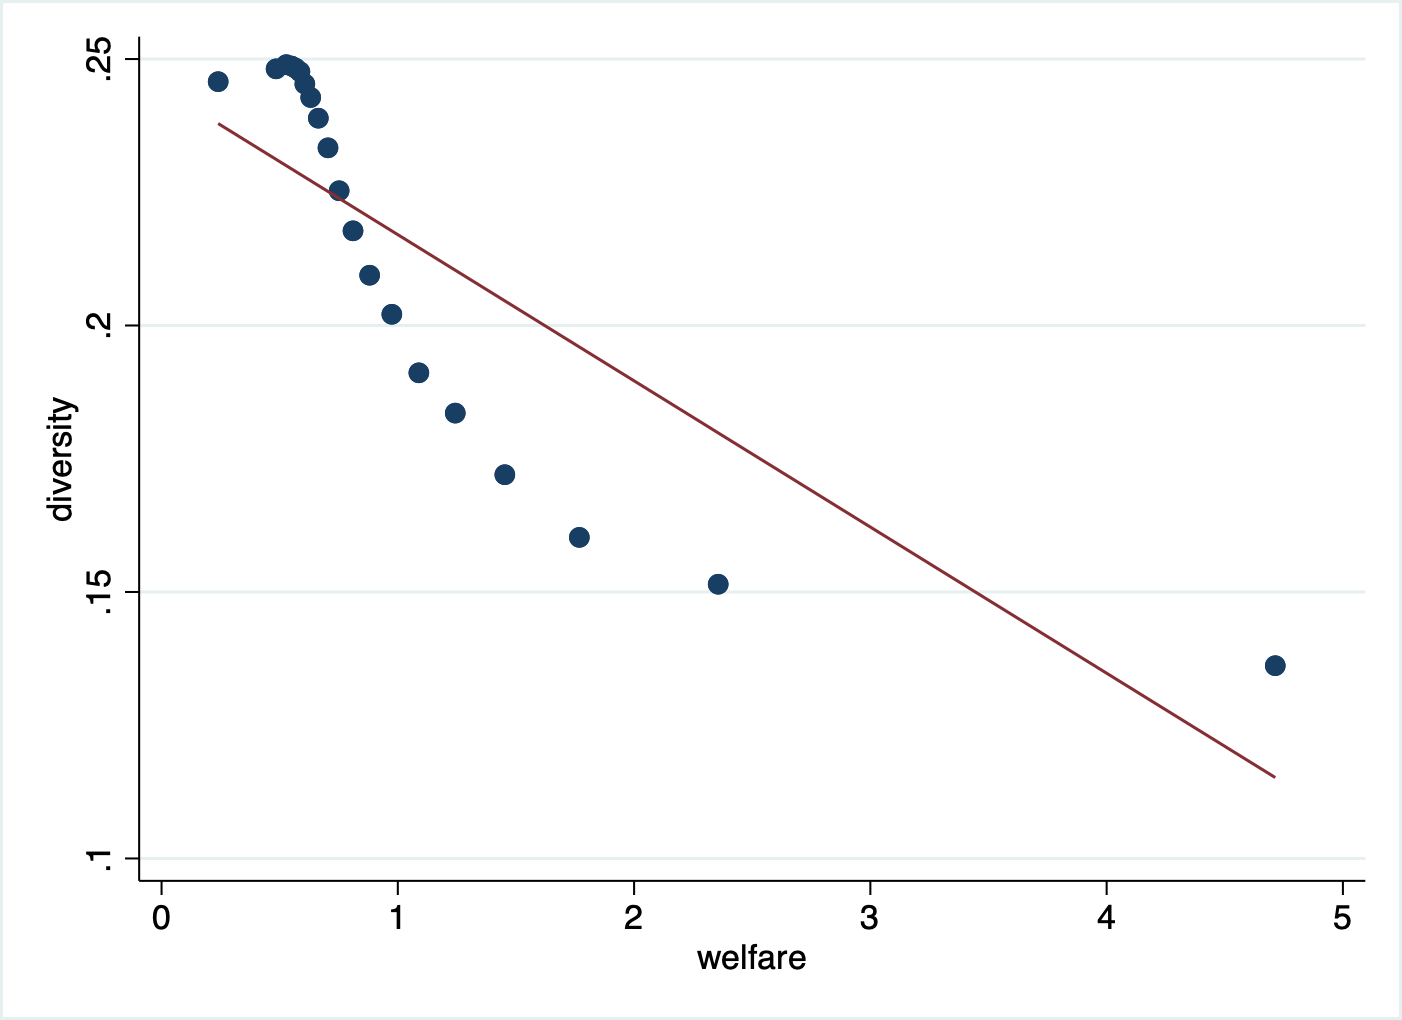
\includegraphics[scale=0.3]{figures/diversity_welfare_no_risk_aversion}
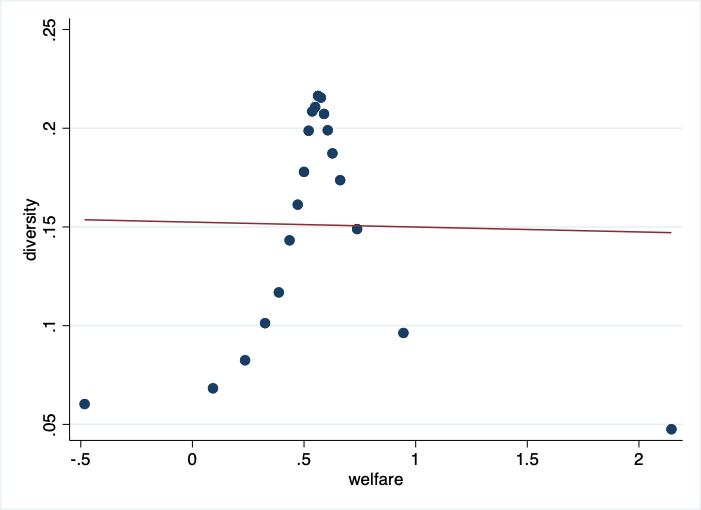
\includegraphics[scale=0.3]{figures/diversity_welfare_high_ra}
\caption{Diversity vs. Welfare, $\gamma = 0$ (Left), Diversity vs. Welfare, $\gamma = 5$ (Right)}
\label{fig:diversity_welfare_ra}
\end{figure*}

\subsection{User Homogenization}

In this section we focus on across user comparisons and investigate how the consumed set of items across users varies across different recommendation regimes and parameter values. In particular we look at the degree of \textit{homogenization} between users. Similar to \cite{chaney2018algorithmic} we use the Jaccard index between the consumption sets of users to measure homogeneity:
\begin{align*}
H:=\frac{1}{|I|(|I|-1)}\sum_{i,j \in I: i \ne j}d_J(C_i^T,C_j^T)
\end{align*}
where $d_J$ denotes the Jaccard index and $H \in [0,1]$.
\begin{finding}\label{finding_homogeneity}
Homogeneity is:
\begin{enumerate}
\item Highest under partial recommendation and lowest under no recommendation
\item Increasing in $\beta$, or the weight of the common-value component
\item Decreasing in $\rho$ for partial recommendation, but weakly increasing in $\rho$ for no recommendation
\end{enumerate}
\end{finding}

Figure \ref{fig:beta_homo} shows that as the weight of the common-value component, $\beta$, increases users consume increasingly similar sets of items. The homogenization effect is strongest under partial recommendation since the revelation of the common-value component induces users to consume products in similar areas of the product space. However, as $\beta$ increases, some amount of homogenization is optimal as can be seen from the omniscient recommendation case. In the no recommendation case since users do not know the common-value component they engage in local consumption in different areas of the product space which leads to less than optimal homogeneity.

Figure \ref{fig:cor_homo} shows that the degree of homogeneity in the partial recommendation case however is \textit{decreasing} as $\rho$ increases. As was discussed in Findings \ref{finding_local_consumption} and \ref{finding_diversity}, the degree of local consumption increases with $\rho$. Even though the revelation of the common-value component induces them to search in similar parts of the product space, their idiosyncratic components induce them to consume products in a more localized area of the product space as $\rho$ increases which leads to a decline in homogeneity.

\begin{figure}
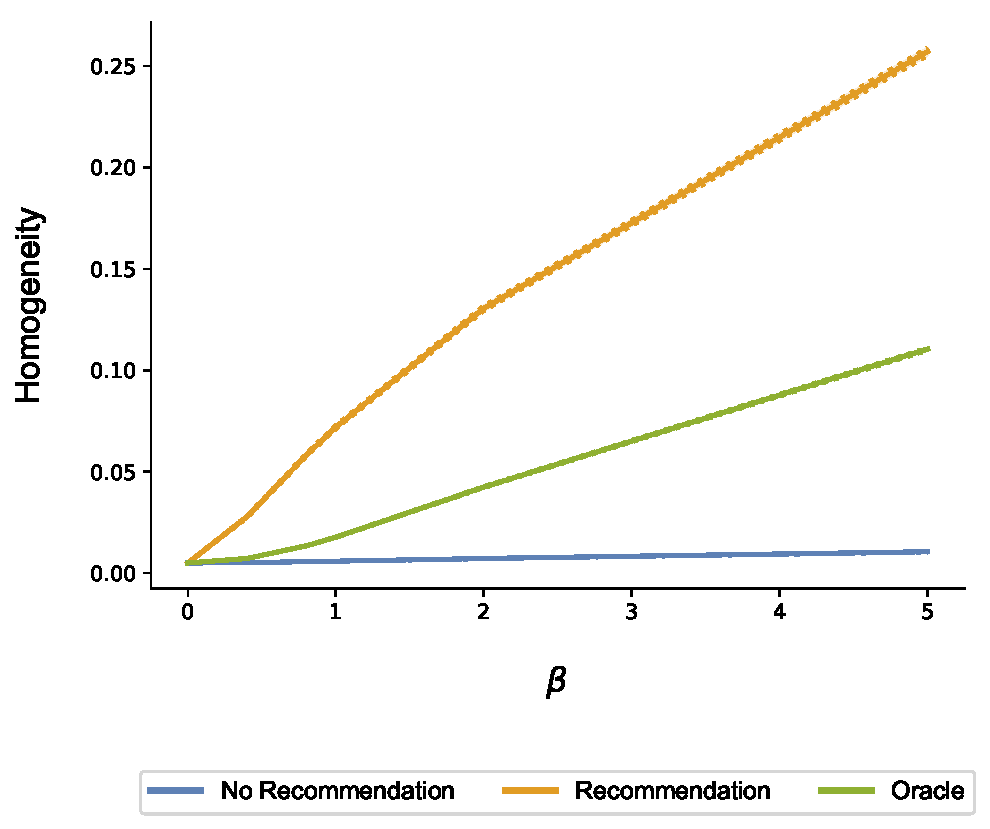
\includegraphics[scale=0.1]{figures/beta_homogeneity_N_200_T_20}
\caption{Strength of Recommendation and Homogeneity}
\label{fig:beta_homo}
\end{figure}

\begin{figure}
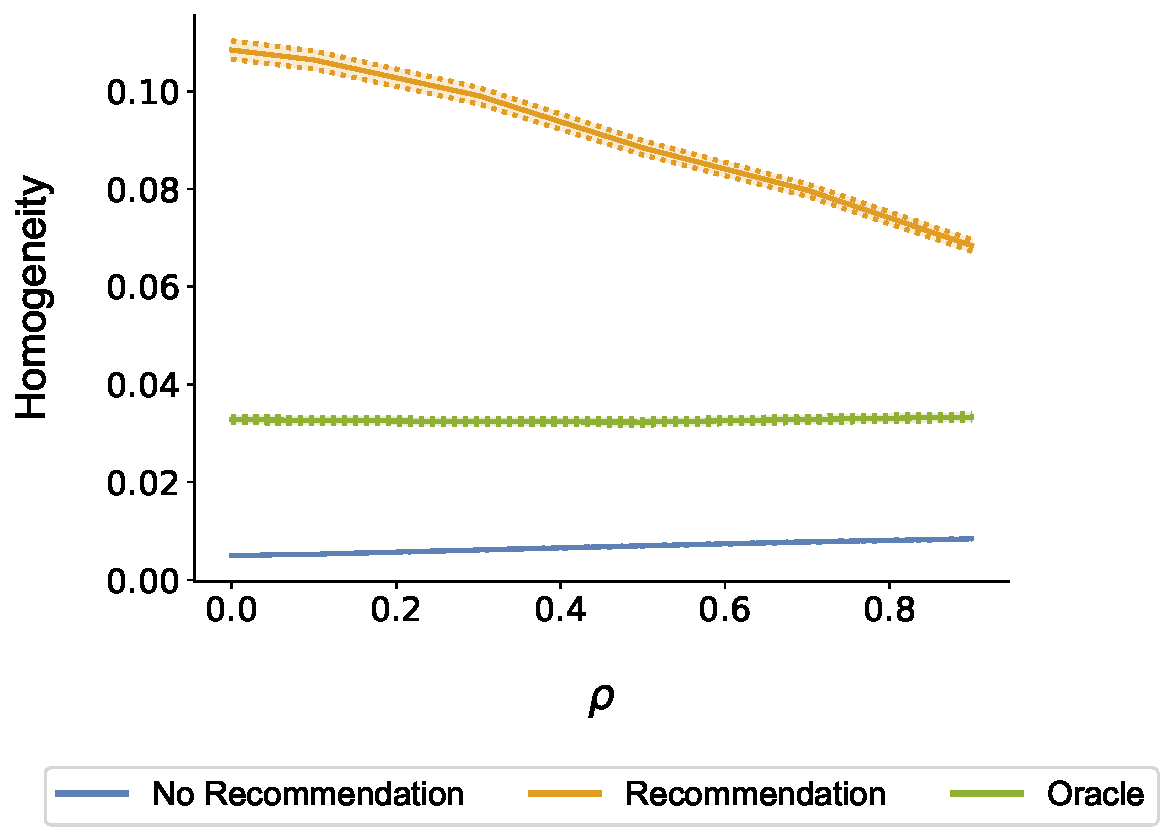
\includegraphics[scale=0.1]{figures/rho_homogeneity_N_200_T_20}
\caption{Correlation and Homogeneity}
\label{fig:cor_homo}
\end{figure}

\section{Recommender System Evaluation}

In this section we discuss how the insights from our model of user decision-making can be used to inform the evaluation and design of recommender systems.

The classic approach to recommender system evaluation is to predict user ratings for items and compare how accurate this prediction is to recorded ratings data, either explicitly given by users or inferred from behavioral data. Further, given this predicted rating, the recommender system should recommend to users the items with the highest predicted rating \cite{adomavicius2005toward}.

There has been a recent movement away from such evaluation measures due to the observation that accurate recommendations are not necessarily useful recommendations \cite{mcnee2006being}. Our model illustrates why this could be the case. Consider the domain of movie recommendation and suppose a user has just watched the movie \textit{John Wick} and rated it highly. A recommender system attempting to predict user ratings may then predict that this user is very likely to enjoy the sequel, \textit{John Wick: Chapter Two}, as well. However, the user themselves may also have made this inference since the two movies are very similar to each other and, after enjoying \textit{John Wick}, the user will update her beliefs about \textit{John Wick: Chapter Two}. Thus, if the recommender system recommends this movie to the user then this recommendation is not useful since the recommendation gives the user little information that they did not already know. As a result, the user may watch \textit{John Wick: Chapter Two} even without recommendation and the value of the recommendation was small.

As a result, several alternative recomendation evaluation metrics, such as serendipity \cite{kotkov2016survey}, coverage \cite{ge2010beyond}, and novelty \cite{vargas2011rank}, have been proposed in order to develop recommender systems that produce recommendations that are more useful for users. We use our model to motivate an alternative recommendation evaluation metric that provides an alternative perspective on the serendipity metric proposed in the literature. Serendipitious recommendations ``have the quality of being both unexpected and useful" \cite{maksai2015predicting}. \cite{iaquinta2010can} defines serendipitous recommendations as follows:
\begin{quote}
\textit{A serendipitous recommendation helps the
user to find a surprisingly interesting item that
she might not have otherwise discovered (or it
would have been really hard to discover). [...]
Serendipity cannot happen if the user already
knows what is recommended to her, because a
serendipitous happening is by definition something new. Thus the lower is the probability that user knows an item, the higher is the
probability that a specific item could result
in a serendipitous recommendation}.
\end{quote}

Our approach to serendipity comes from the intuition that a recommendation is only useful insofar as it leads a user to take a better action than she would without recommendation. This approach stems from the idea that the value of recommendation is the marginal gain in expected utility that a user receives from recommendation.\footnote{This notion is similar to the ``value of information" notion utilized in the literature in economics on the pricing of information goods \cite{bergemann2018design}.} This intuitively should come from providing information about products that, without additional information, users assign a low likelihood to being the best product currently available and so would not consume them without recommendation.

This differs from other approaches in the literature since it depends on the beliefs of the users and what item the user would consume without recommendation. For instance, \cite{vargas2011rank, kaminskas2014measuring} propose unexpectedness metrics that look at the dissimilarity of the recommended items to what the recommender already knows the user likes either via a content-based approach or a collaborative-based approach. This depends only on the resulting item-set that the users get recommended and not necessarily user beliefs or the change in user action. \cite{adamopoulos2015unexpectedness} use an expected utility approach but use this to measure unexpectedness in terms of deviations from the ``expected consideration set" of a user and do not explicitly incorporate user beliefs.

Our model allows us to give precise definitions for what it means for a recommendation to be \textit{unexpected} and \textit{useful}. Unexpected recommendations are given by recommended items that, given their beliefs, users have low expected utility from consuming, irregardless of what the true realized utility is. Recall from Findings \ref{finding_local_consumption} and \ref{finding_diversity_welfare_corr} that, particularly if users are risk-averse, they will consume content in increasingly narrow portions of the product space and this may be detrimental to their realized welfare. As a result, identifying the portions of the product space where users may have significant uncertainty and utilizing recommendation to reduce this uncertainty can be welfare-enhancing for users. This is especially the case if this reduction of uncertainty leads users to explore under-explored portions of the product space where true realized utility is high, but expected utility, given beliefs, is low before recommendation.

Useful recommendations are recommendations that give users information that would change the item they consume relative to no recommendation and lead to an increase in expected utility. In the previous example, recommending \textit{John Wick: Chapter Two} is not useful precisely because the expected utility before and after recommendation is the same since it does not change behavior. The most useful recommendations, or those that have the highest utility gain, are recommendations that induce users to consume unexpected goods.

Operationalizing this approach requires the collection of data that is not traditionally collected for recommender systems. In particular, it becomes important to understand what choices users would make \textit{without recommendation} and to collect data on user beliefs, which can partially be inferred by observed choices. \cite{jiang2014choice, saavedra2016choice} argue that choice-based approaches alone can help in designing better RS, though they argue for these approaches because they do a better job at providing more accurate recommendations. However, we argue that choice-based approaches are useful not as recommendations but as a baseline for what recommendations would be useful.\footnote{Furthermore, user beliefs and user choices contain information that may not have been observed by the recommender but is observed by the user. Ratings, reviews, friends, there are many sources of information affecting a person's beliefs and choices that are unobservable by recommender systems. Other consumption choices, e.g. movies seen in the cinema, change beliefs about for instance how good a director is, which affect beliefs about other movies and guide choices on a streaming platform that is unable to observe these data. However, this information can be inferred by the platform by collecting both beliefs and consumption choices.}

Furthermore, our model shows the importance of understanding the underlying user preferences and the nature of the product space in the setting in which a recommender system is deployed since that will change the consumption patterns of users. For instance, understanding the degree of correlation of utilities and the level of risk-aversion become crucial in understanding how users will make consumption choices without recommendation and what kind of recommendation would be useful for users.

\section{Discussion}

\section{Conclusion}

We have argued that incorporating user choice under uncertainty should be a first-order component of RS design. By collecting appropriate data about user choices and user beliefs, RS can be built to better understand what choices users are likely to make and thus what information would be useful to give them as opposed to simply predicting what items a user will like. This approach can not only aid in designing more useful RS, but can also be utilized to better understand and prevent recently documented adverse effects of RS such as filter bubbles and homogenization.

\bibliographystyle{plain}
\bibliography{refs}
\end{document}
